% !TEX program = xelatex
\documentclass[12pt,a4paper]{article}

%%
% CUMCM 数学建模竞赛论文写作培训模板（2026规范+AI规定内嵌版）
% 用法：本文件既可作为培训讲义，也可作为参赛论文写作母版。
% 正式参赛时：删除所有“【培训提示】”文字、示例性内容，并替换为本队实际内容。
% 本版本已嵌入用户实际论文内容，并保留全部培训注释与提示，便于修改验证。
%%

\usepackage{geometry}
\geometry{a4paper,left=2.5cm,right=2.5cm,top=2.5cm,bottom=2.5cm}
\usepackage{ctex}
\usepackage{sectsty}
\sectionfont{\centering}
\renewcommand\thesection{\chinese{section}、}
\renewcommand\thesubsection{\arabic{section}.\arabic{subsection}}
\usepackage[dvipsnames]{xcolor}
\usepackage{booktabs}
\usepackage{makecell}
\usepackage{amsfonts,amsmath,amssymb,mathtools}
\usepackage{multirow}
\usepackage{graphicx}
\graphicspath{{figures/}}
\usepackage{subcaption}
\usepackage{float}
\usepackage{enumitem}   
\usepackage{array}
\usepackage{longtable}
\usepackage{listings}
\usepackage{fancyvrb}
\usepackage{algorithm}
\usepackage{algpseudocode}
\usepackage{fancyhdr}
\usepackage{hyperref}
\usepackage{url}

\hypersetup{
  colorlinks=true,
  linkcolor=black,
  urlcolor=blue,
  citecolor=black,
  pdfstartview=Fit,
  breaklinks=true
}

\lstset{
  frame=tb,
  aboveskip=3mm,
  belowskip=3mm,
  showstringspaces=false,
  columns=flexible,
  framerule=1pt,
  rulecolor=\color{gray!35},
  backgroundcolor=\color{gray!5},
  basicstyle={\small\ttfamily},
  numbers=left,
  numberstyle=\tiny\color{gray},
  keywordstyle=\color{blue},
  commentstyle=\color{ForestGreen},
  breaklines=true,
  breakatwhitespace=true,
  tabsize=3
}
\renewcommand{\lstlistingname}{源程序}

\newcommand{\tip}[1]{\par\noindent\textbf{【提示】} #1\par}
\newcommand{\warning}[1]{\par\noindent\textbf{【高频失分点】} #1\par}
\newcommand{\good}[1]{\par\noindent\textbf{【推荐写法】} #1\par}
\newcommand{\bad}[1]{\par\noindent\textbf{【不推荐写法】} #1\par}
\newcommand{\core}[1]{\boxed{\text{#1}}}

\fancyhf{}
\cfoot{\thepage}
\renewcommand{\headrulewidth}{0pt}
\pagestyle{fancy}

\begin{document}

% ============================================================
% 摘要页：电子版第一页，页码从1开始
% ============================================================
\pagenumbering{arabic}
\setcounter{page}{1}

\begin{center}
{\zihao{-2}\bfseries 多火箭残骸音爆定位模型}

\vspace{2ex}
{\zihao{3}\bfseries 摘要}
\end{center}

本文针对多级火箭分离后多个残骸在坠落过程中产生跨音速音爆的定位问题，建立了从“单事件到达时间定位”到“多事件数据关联与联合定位”再到“带随机时间误差的稳健定位”的一整套模型。首先将经纬度按题目给定比例转换为局部平面坐标，把每个音爆事件抽象为位置与时刻均为未知的瞬时声源，得到到达时间方程；再通过时间差（TDOA）消去音爆时刻，将问题化为非线性最小二乘反演。

针对问题1，未知量为经度、纬度、高程、音爆时刻，根据方程可解性定理可以得到结论：单个残骸的精确反演至少需要 4 台设备。为解决出现多解的情况，应使用大于4台设备。针对 7 台设备的算例，本文先利用两两到达时间差的几何必要条件对数据做一致性筛选，剔除与同一声事件明显不自洽的记录，再采用带多初值的高斯——牛顿法与列文伯格——马夸尔特法求解，得到该残骸音爆位置约为 $110.7164^\circ\mathrm{E}$、$27.0297^\circ\mathrm{N}$，高程约 18663 m，音爆时刻约 $-38.03$ s，所选四台设备的残差平方和 $SSE\approx 0$。
% 【以下为与上文重复的表述，保留备查】
% 先利用两两到达时间差的几何必要条件 $c|t_i-t_j|\le\|S_i-S_j\|$ 对数据作一致性筛选，再从可行组合中选取内部自洽的 BDFG 四台设备，采用带多初值的高斯--牛顿法与列文伯格--马夸尔特法求解。

在问题2中，引入每台设备的关联排列 $\sigma_i$，将“哪一次记录属于哪一个残骸”建模为离散排列变量，并与 16 个连续参数（4 个残骸的位置与时刻）共同构成混合优化模型。若波的归属未知，4 台设备只能得到 16 个观测、恰好等于 16 个连续未知量，无法判别错误关联；需要 $4N>16$，也就是至少 5 台设备，才能利用超定残差唯一确定关联。

对于问题3，本文采用“固定关联—分别定位”与“固定位置—匈牙利算法更新关联”的交替迭代求解，结合“四个音爆时刻相差不超过 5 s”的约束筛选，解出四个残骸的位置、高程与音爆时刻；所给四组解的全部 28 个到达时间残差均小于 $6\times10^{-4}$ s，与表中三位小数的记录精度一致，验证了关联与定位结果的正确性。

针对问题4，将到达时间误差建模为$U(-0.5,0.5)$均匀分布的随机误差，把问题2的模型修正为加权最小二乘联合优化，并给出蒙特卡洛误差分析：在 7 台设备、关联正确的条件下，500 次试验中四个残骸三维定位误差均值约为 230-730 m；若进一步将台站加密到 12 台并优化布局，总体平均误差约 225 m、95\% 分位数约 532 m，可实现“误差小于 1 km”的目标。

模型的优点在于把“数据关联”与“几何定位”统一在一个目标函数中求解，并用一致性检验、残差分析与蒙特卡洛试验形成完整验证链；通过增加台站数、改善几何布局或引入弹道约束，还可进一步抑制时间误差的影响。

\vspace{2ex}
\noindent{\heiti 关键词：} 音爆定位；最小二乘法非线性规划；匈牙利算法；混合优化；蒙特卡洛误差分析

% \vspace{2ex}
% \tip{摘要专用页原则上不超过一页；摘要、正文、附录中任何地方都不能出现参赛者身份、所在学校及赛区信息；页码从摘要页开始，以阿拉伯数字1连续编号，位于页脚中部。不写英文摘要。摘要不是“目录式介绍”，而是一页内让评阅人回答四个问题：\textbf{研究什么、怎么建模、怎么求解、得到什么结论}。  

% 一个好摘要至少应出现若干“可核验”的结果，例如“预测误差降低至X\%”“最优方案使成本下降X\%”“温度峰值达到X℃”“准确率为X\%”。如果全文最有价值的结论没有进入摘要，评阅人很容易错过论文亮点。}

% \begin{table}[H]
% \centering
% \caption{摘要逐句检查表}
% \begin{tabular}{p{2.8cm}p{10.5cm}}
% \toprule
% 句子功能 & 应回答的问题 \\
% \midrule
% 背景与目标 & 现实问题是什么？本文究竟解决什么？ \\
% 模型概述 & 建立了什么模型？核心变量和关系是什么？ \\
% 求解方法 & 用什么算法/理论方法？为什么适合？ \\
% 主要结果 & 最重要的数值、排序、趋势或最优方案是什么？ \\
% 结论与应用 & 结果说明什么？能用于什么决策？ \\
% \bottomrule
% \end{tabular}
% \end{table}

% \warning{摘要中避免“本文首先$\cdots$其次$\cdots$最后$\cdots$”连续堆砌过程，却不明确写出算出了什么；避免“结果很好、模型合理、效果显著”等没有数据支撑的空泛表述。}

\clearpage

% ============================================================
% 一、问题重述
% ============================================================
\section{问题重述}

% \tip{问题重述的任务不是“复印题目”，而是把题目翻译成数学建模语言。建议压缩原题背景，保留真正影响模型的条件、目标和输出。}

\subsection{问题背景}

多级火箭在飞行过程中会分离下面级火箭和助推器，这些分离的残骸在下落过程中会穿越音速附近，产生跨音速音爆。在理论落区布置监测设备即可记录各残骸音爆到达的时刻。利用各级残骸的到达时间，就能反演残骸发生音爆时的空间位置与时刻。结合弹道外推估计落点即可为快速回收提供依据。

多残骸场景中，单台设备无法得知第几组波来自哪一个残骸，需要结合多台设备来进行分析。

因此，本问题含有两方面的挑战：一是“定位”，即求解残骸音爆的空间位置与时刻；二是“数据关联”，即判别每台设备收到的波属于哪一个残骸。

\subsection{问题重述}

（1）根据物理条件建立数学模型，分析空中单个残骸发生音爆时的经度、纬度、高程与时间所需的最少设备数，并从7台设备的数据中选取合适的数据，计算该残骸发生音爆的位置与时间。
% 【以下原句中的“发震时刻”等措辞与本文无关，保留备查】
% 即根据多站到达时延建立非线性最小二乘反演模型，求解声源坐标与发震时刻。

（2）假设空中有4个残骸，每个设备按时间先后收到4组震动波。建立模型确定每组波属于哪一个残骸，并回答确定4个残骸位置与时间所需的最少设备数，即在未知“波—源”归属关系的条件下，将离散关联变量与连续定位参数纳入统一的混合优化模型进行联合求解。

（3）利用7台设备各4组到达时间的数据，解出4个残骸的经度、纬度、高程与音爆时刻，其中四个音爆时刻相差不超过5s，即在完成数据关联后，对每个残骸分别进行多站时差定位，并以音爆时刻的时序一致性作为物理约束筛选合理关联。

（4）假设设备记录时间存在0.5s的随机误差，修正问题2的模型并给出带误差算例与误差分析。如果时间误差无法降低，提出实现误差小于1km的定位方案，并依据问题3结果模拟布站与观测数据加以验证，即通过蒙特卡洛方法量化随机误差对定位精度的影响，并通过增加台站与优化几何布局提升系统稳健性，使三维定位误差稳定控制在1km以内。

% \begin{table}[H]
% \centering
% \caption{问题重述的四要素}
% \begin{tabular}{p{3cm}p{10cm}}
% \toprule
% 要素 & 写作内容 \\
% \midrule
% 已知条件 & 数据、边界、物理规律、题目给定约束 \\
% 决策变量 & 哪些量可以控制、优化或预测 \\
% 模型任务 & 拟合、预测、分类、评价、优化、调度、仿真等 \\
% 输出结果 & 数值、排序、最优方案、策略、敏感因素等 \\
% \bottomrule
% \end{tabular}
% \end{table}

% \warning{绝对避免大段照抄题面。即使没有查重要求，照抄也会浪费正文篇幅，并且无法体现建模能力。}

% ============================================================
% 二、问题分析
% ============================================================
\section{问题分析}

% 这一部分体现“从实际问题到数学问题”的思维过程。核心不是介绍算法，而是解释\textbf{为什么这样建模}。

% \[
% \boxed{\text{题目给了什么？}\quad\text{真正难点是什么？}\quad\text{准备怎样把它数学化？}}
% \]

% \tip{问题分析通常控制在每个问题4--10行，但信息密度要高。不要在这里提前公布详细计算结果；模型公式放到后面的“模型建立”。}

\subsection{问题1的分析}

单个残骸发生音爆时，位置需要 3 个坐标描述，加上 1 个音爆时刻，共 4 个未知量。每台设备只提供 1 个到达时刻，因此从自由度上至少需要 4 台设备。但到达时间方程是非线性的，4 台设备在数学上可能出现两个镜像解，且测量误差会被放大；因此理论下限是 4 台，实际求解应采用更多设备形成超定方程组。

对于给出的 7 台数据，先利用“同一事件在两台设备上的时间差不可能超过两台设备间距除以声速”这一必要条件做数据体检，再从一致的数据中选择/组合求解，最后用全部台站残差交叉验证，避免个别异常记录污染定位结果。

\subsection{问题2的分析}

问题2在问题1的基础上增加“数据关联”这一离散层：每台设备收到的 4 组波按时间先后排列，但不同残骸到不同设备的传播距离不同，所以“先听到”不代表“先发生”，同一残骸在各设备中的到达顺序也可能不同。不能简单地把所有设备第 $k$ 早的波归为一组。

因此把关联变量建模为排列，将离散关联与连续位置时刻放入同一个残差平方和目标函数。求解时采用“固定关联—定位”与“固定位置—指派”的交替迭代。设备数方面，需要同时比较未知量数与观测数：4 台设备时观测数恰等于连续未知量数，无法判别关联，5 台设备才使系统超定。

\subsection{问题3的分析}

问题3给出 7 台设备、每台 4 个到达时间。应先恢复“哪个波属于哪个残骸”的关联矩阵，再对每个残骸分别执行问题1的定位。利用四个音爆时刻相差不超过 5 s、位置落在合理空域等物理约束可以大幅缩小候选关联的搜索范围，最终以“28 个到达时间全部自洽”作为验证标准。

\subsection{问题4的分析}

0.5 s 的时间误差折算为距离约 170 m，会同时影响定位精度与关联判断。因此需要把问题2模型中的普通最小二乘修正为加权最小二乘，并在关联层使用残差假设检验；通过蒙特卡洛试验统计位置误差。若时间误差无法进一步降低，则应通过增加台站、优化几何布局、引入弹道与四残骸之间的时间约束等方式换取空间冗余，从而实现 1 km 精度。

% ============================================================
% 三、模型假设
% ============================================================
\section{模型假设}

% \tip{好的假设不是越多越好，而是“必要、合理、可解释、能降低复杂度”。每一个关键假设最好能回答：为什么需要？违反它会怎样？是否会影响结论？} 常见假设来源：
% \begin{enumerate}[label=(\arabic*)]
%   \item 题目明确给出的条件；
%   \item 排除极低概率或明显异常事件；
%   \item 忽略对目标影响很小的次要因素；
%   \item 某经典模型或算法所要求的技术假设；
%   \item 对未知参数、分布、噪声形式作合理假设；
%   \item 为使模型可计算而进行的合理离散化或近似。
% \end{enumerate}

% \begin{table}[H]
% \centering
% \caption{模型假设的推荐写法}
% \begin{tabular}{p{2cm}p{5cm}p{6cm}}
% \toprule
% 假设类型 & 不推荐 & 推荐 \\
% \midrule
% 数据异常 & 数据没有问题 & 剔除明显录入错误及超出物理范围的异常点，并保留处理规则 \\
% 次要因素 & 其他因素忽略 & 经量纲/数量级分析，次要因素相对于主导因素影响可忽略 \\
% 随机性 & 假设数据服从正态分布 & 通过QQ图/检验/领域知识说明采用该分布的依据 \\
% 简化 & 为了方便计算 & 在不改变主要趋势和核心约束的前提下进行合理简化 \\
% \bottomrule
% \end{tabular}
% \end{table}

% \warning{不要把“假设模型结果正确”“假设结果符合预期”写进模型假设。这是循环论证。}

\begin{enumerate}[label=(\arabic*)]
  \item 声速恒定，取 $c=340$ m/s，忽略声速随温度、高度与风速的变化；
  \item 计算两点间距离时忽略地面曲率，经度每度按 $97.304$ km、纬度每度按 $111.263$ km 换算为平面距离；
  \item 每个残骸的一次音爆可视为一个瞬时声源事件，声波沿直线以球面波形式传播；
  \item 各台监测设备时钟已同步，到达时间记录相互可比；
  \item 第 $i$ 台设备收到的 4 组震动波恰好来自 4 个不同的残骸，即每个残骸在该设备上只产生一个到达记录；
  \item 在问题4中，各设备记录时间误差相互独立，误差上限为 0.5 s；
  \item 残骸音爆点在落区附近合理空域内，音爆时刻不晚于其对应的到达时刻。
\end{enumerate}

% ============================================================
% 四、符号说明
% ============================================================
\section{符号说明}

% \tip{只列核心变量。临时求和指标、简单中间变量不必全部塞进符号表，但正文首次出现时仍应解释。符号应尽量有含义，避免同一个字母在不同章节代表不同变量。}

\begin{table}[H]
\centering
\caption{主要符号说明}
\label{tab:symbol}
\begin{tabular}{p{3cm}p{8cm}p{2cm}}
\toprule
符号 & 说明 & 单位\\
\midrule
$i$ & 监测设备编号 & -- \\
$d$ & 残骸编号 & -- \\
$S_i=(x_i,y_i,h_i)$ & 第 $i$ 台设备坐标（经纬度换算为平面坐标） & m \\
$P_d=(x_d,y_d,h_d)$ & 残骸 $d$ 音爆点位置 & m \\
$\tau_d$ & 残骸 $d$ 的音爆时刻 & s \\
$t_{i,k}$ & 第 $i$ 台设备第 $k$ 早到达时刻 & s \\
$t_{i,\sigma_i(d)}$ & 分配给残骸 $d$ 的实测到达时刻 & s \\
$\sigma_i$ & 第 $i$ 台设备的关联排列 & -- \\
$y_{i,k,d}$ & 0-1 关联变量 & -- \\
$c$ & 声速 & m/s \\
$\varepsilon$ & 记录时间随机误差 & s \\
\bottomrule
\end{tabular}
\end{table}

% \tip{符号设计的经验：优先使用约定俗成记号；没有约定时可用英文含义前缀，如 $T_{\max}$、$T_{\mathrm{tol}}$、$C_{\mathrm{cost}}$；关键决策变量可直接使用 $x_i$。不要为了“高级”而使用过于复杂的希腊字母。}

% ============================================================
% 五、模型建立与求解
% ============================================================
\section{模型的建立与求解}

% \tip{这是全文核心。评阅人真正关心的是：从题目条件怎样得到数学关系？模型是否闭合？变量、参数、约束、目标是否定义清楚？算法能否真正求出这个模型？}

% \subsection{建模总路线：从文字到公式}% 空小节标题，正文未使用，保留备查

% \[
% \boxed{
% \text{题目条件}
% \rightarrow
% \text{变量定义}
% \rightarrow
% \text{基本规律}
% \rightarrow
% \text{数学关系}
% \rightarrow
% \text{约束}
% \rightarrow
% \text{目标函数}
% \rightarrow
% \text{完整模型}
% }
% \]

% \begin{table}[H]
% \centering
% \caption{不同题型的核心模型结构}
% \begin{tabular}{p{3cm}p{11cm}}
% \toprule
% 题型 & 论文中必须交代的核心内容 \\
% \midrule
% 预测 & 数据预处理、特征、模型、训练/拟合、误差指标、预测结果 \\
% 评价 & 指标体系、权重、标准化、综合评价、稳健性检验 \\
% 优化 & 决策变量、目标函数、约束、求解算法、最优方案 \\
% 分类 & 特征、标签、训练策略、评价指标、分类结果 \\
% 聚类 & 距离/相似度、类别数、聚类算法、稳定性、类别解释 \\
% 微分方程 & 状态变量、机理方程、初边值条件、参数、数值方法 \\
% 图论/网络 & 节点、边、权重、路径/流/连通性定义及算法 \\
% \bottomrule
% \end{tabular}
% \end{table}

\subsection{公共几何框架}

我们设定模型整体都以 $(110^\circ\mathrm{E},\ 27^\circ\mathrm{N})$ 为参考点，由于忽略地面曲率，且纬度间每度距离值近似为111.263 km，经度间每度距离值近似为97.304 km，可以把经度、纬度差转换为米制平面坐标：
\[
x_i=(\lambda_i-110)\times 97304,\qquad
y_i=(\varphi_i-27)\times 111263.
\]

若残骸$d$在 $P_d$ 于时刻 $\tau_d$ 发生音爆，则第 $i$ 台设备到达时间为
\[
t_{id}=\tau_d+\frac{\|P_d-S_i\|}{c},
\]
其中
\[
\|P_d-S_i\|=\sqrt{(x_d-x_i)^2+(y_d-y_i)^2+(h_d-h_i)^2}.
\]
化简得到方程
\begin{equation}
\|P_d-S_i\|^2=c^2\left(t_{id}-\tau_d\right)^2.
\end{equation}\label{eq1}

下面详细推导便于数值求解的线性化形式。把方程 \eqref{eq1} 展开，记
$P_d=(x_d,y_d,h_d)$，$S_i=(x_i,y_i,h_i)$，得到
\begin{equation}
\|P_d\|^2-2P_d\cdot S_i+\|S_i\|^2
=c^2\left(t_i^2-2t_i\tau_d+\tau_d^2\right).
\end{equation}
对第 $r$ 台设备写同样的展开式，并与上式相减。等式两侧的 $\|P_d\|^2$ 与 $c^2\tau_d^2$ 同时消去，得到
\begin{multline}
-2P_d\cdot\left(S_i-S_r\right)+\left(\|S_i\|^2-\|S_r\|^2\right)\\
=-2c^2\tau_d\left(t_i-t_r\right)+c^2\left(t_i^2-t_r^2\right).
\end{multline}
整理后，对每一对设备 $(i,r)$ 都可以得到关于 $(x_d,y_d,h_d,\tau_d)$ 的线性方程
\begin{equation}
\begin{aligned}
&(x_i-x_r)x_d+(y_i-y_r)y_d+(h_i-h_r)h_d-c^2(t_i-t_r)\tau_d\\
&=\frac12\left[\|S_i\|^2-\|S_r\|^2-c^2\left(t_i^2-t_r^2\right)\right].
\end{aligned}
\end{equation}
若用固定参考台站 $r$ 与其余 $N-1$ 台设备构造方程，则得到
\begin{equation}
A\theta=b,\qquad \theta=(x_d,y_d,h_d,\tau_d)^\top.
\end{equation}
这是关于未知量的\textbf{线性方程组}，可直接用最小二乘求初值。注意到上述推导来自“方程相减”，理论上可能混入由两边平方带来的符号问题，因此线性解只作为初值，最终仍用未平方的到达时间残差做非线性精化。对任意两台设备，残差还必须满足三角形不等式
\[
c|t_{id}-t_{rd}|\le\|S_i-S_r\|,
\]
该必要条件可用于数据一致性筛选与关联剪枝。

\subsection{算法概述}

\subsubsection{非线性最小二乘与高斯--牛顿法}

设待估参数为 $\theta$，残差向量为
\[
r(\theta)=\left(r_1(\theta),\dots,r_m(\theta)\right)^\top,
\]
其中 $m$ 为方程个数。目标函数为
\[
F(\theta)=\frac12\sum_{k=1}^{m}r_k^2(\theta)=\frac12 r^\top r.
\]
若在 $\theta^{(n)}$ 附近作一阶泰勒展开，令
\[
J_{kj}=\left.\frac{\partial r_k}{\partial \theta_j}\right|_{\theta^{(n)}},
\]
得到线性化近似 $r(\theta^{(n)}+\Delta)\approx r(\theta^{(n)})+J\Delta$。将其代入 $F$，对 $\Delta$ 求极小可得\textbf{高斯--牛顿法}的迭代方程
\begin{equation}
\left(J^\top J\right)\Delta=-J^\top r.
\end{equation}
由于到达时间模型强非线性，$J^\top J$ 可能接近奇异或导致步长过大。为此加入阻尼项 $\mu>0$，即列文伯格--马夸尔特法：
\begin{equation}
\left(J^\top J+\mu I\right)\Delta=-J^\top r,
\end{equation}
并迭代更新 $\theta^{(n+1)}=\theta^{(n)}+\Delta$。阻尼项越大，步长越保守；残差下降时减小 $\mu$，残差不降或上升时增大 $\mu$。收敛准则可取
\[
\|J^\top r\|_{\infty}<\varepsilon_1,\qquad
\|\Delta\|<\varepsilon_2.
\]
由于目标函数非凸，应从多组初值出发，保留总残差最小且满足物理约束的解。

\subsubsection{求解单事件定位}

\begin{algorithm}[H]
\caption{单事件定位：线性初值 + 列文伯格--马夸尔特迭代精化}
\label{alg:single}
\begin{algorithmic}[1]
\Require 监测台站集合 $\{S_i\}$、到达时刻 $\{t_i\}$、声速 $c$
\Ensure 音爆点参数 $\theta=(x,y,h,\tau)$
\State 选取参考台站 $r$，由两两相减方程构造线性系统 $A\theta=b$
\State 用线性最小二乘求初值 $\theta^{(0)}$
\State 初始化阻尼 $\mu\leftarrow\mu_0$，迭代次数 $n\leftarrow0$
\Repeat
  \State 计算残差向量 $r(\theta^{(n)})$ 与雅可比矩阵 $J(\theta^{(n)})$
  \State 求解 $(J^{\top}J+\mu I)\Delta=-J^{\top}r$
  \If{目标残差下降}
    \State 更新 $\theta^{(n+1)}\leftarrow\theta^{(n)}+\Delta$，并减小 $\mu$
  \Else
    \State 增大 $\mu$ 并重新求解 $\Delta$
  \EndIf
  \State $n\leftarrow n+1$
\Until{满足 $\|J^{\top}r\|_{\infty}<\varepsilon$ 或 $n\ge N_{\max}$}
\State 更换多组初值，重复上述迭代
\State 返回总残差最小且满足物理约束的解 $\theta^{*}$
\end{algorithmic}
\end{algorithm}

算法~\ref{alg:single} 中的线性系统用于获得初值，LM 迭代负责精化；由于残差平方和非凸，必须配合多初值策略，避免停留在局部最优。

\subsubsection{匈牙利算法（指派问题）}

在“给定位置求关联”时，需要把 4 个预测到达时间与 4 个实测到达时间一一配对，使代价最小，属于标准指派问题。匈牙利算法步骤如下：

\begin{enumerate}[label=\arabic*.]
  \item 对代价矩阵每一行减去该行最小值；
  \item 对所得矩阵每一列减去该列最小值；
  \item 用最少的横线/竖线覆盖全部零元素；
  \item 若覆盖线数等于阶数，则可选出每行每列各一个零，得到最优指派；
  \item 若覆盖线数小于阶数，取所有未被覆盖元素中的最小值，未被覆盖元素减该值，交叉点加该值，然后回到第 3 步。
\end{enumerate}

原理是：给某一行或某一列整体加常数只会让所有可行方案的总代价同时改变同一常数，因此最优指派不变；调整矩阵只为了让矩阵出现足够多的零，从而从零中选出最优方案。

\subsection{问题1：单个残骸定位模型}

\subsubsection{最少设备数}

未知量有：$x_d,y_d,h_d,\tau_d$，一共 4 个。根据方程组可解性理论，要想唯一确定未知量，需要的方程数等于未知数的个数，因此至少需要\textbf{四台设备}。

然而，根据\ref{eq1}方程的次数为2，因此有可能出现两个镜像解。为了保证解的唯一性，实际使用中至少需要5台。当然，也可以借助物理约束、常用数据（例如常见的一级火箭分离高度）剔除错误分支。本题一共提供7个设备的数据，可构造超定方程组以最小二乘求解。

\subsubsection{定位模型}

取 7 台设备的观测值，定义残差为实际距离与预测距离之差：
\begin{equation}
  r_i=\|P-S_i\|-c(t_i-\tau),
\end{equation}\label{eq2}

问题1的求解目标变为求解非线性最小二乘问题：
\begin{equation}
  \min_{x,y,h,\tau}\ \sum_{i=1}^{7}r_i^2.
\end{equation}\label{eq3}

求解过程中，根据两台设备的方程线性化得到初值，再用高斯——牛顿法或列文伯格——马夸尔特法迭代精化，从多组初值出发取到全局最优。

\subsubsection{数据一致性检验与求解结果}

对任意两台设备 $i,j$，假设同一个残骸在某个位置于时刻 $\tau$ 发生音爆，声音以声速 $c$ 传播，残骸到第 $i$ 台设备和第 $j$ 台设备的距离分别为 $d_i$、$d_j$，可以得到两台设备收到的时间为：
$$t_i=\tau+\frac{d_i}{c}$$
$$t_j=\tau+\frac{d_j}{c}$$
两式相减以消去音爆时刻 $\tau$，得到：
$$c(t_i-t_j)=d_i-d_j$$
两设备间的距离为 $\|S_i-S_j\|$，根据三角不等式可得：
\begin{equation}
  c|t_i-t_j|\le\|S_i-S_j\|.
\end{equation}
为说明“选取合适的数据”的具体过程，本文按 4 台设备一组对可行组合进行一致性检验与最小二乘定位，结果见表~\ref{tab:q1comb}。表中 $SSE$ 为定位方程的残差平方和，若 $SSE$ 接近零，说明该组合的四条到达时间方程内部自洽。

\begin{table}[H]
\centering
\caption{4 台组合的一致性检验与定位结果}
\label{tab:q1comb}
\begin{tabular}{lcccccc}
\toprule
组合 & SSE ($\mathrm{s}^{2}$) & 经度 ($^{\circ}$) & 纬度 ($^{\circ}$) & 高程 (m) & $t_{0}$ (s) \\
\midrule
BDFG & 0.0000 & 110.7164 & 27.0297 & 18663 & -38.03 \\
ABEG & 0.0988 & 110.4978 & 27.3143 & 1154  & 19.09 \\
ABCG & 0.1317 & 110.5064 & 27.3002 & 1138  & 18.79 \\
ACEG & 0.2691 & 110.4658 & 27.3332 & 1097  & 24.15 \\
ABDF & 3.6397 & ---      & ---      & ---   & --- \\
ABCE & 5.8638 & ---      & ---      & ---   & --- \\
\bottomrule
\end{tabular}
\end{table}

由表~\ref{tab:q1comb} 可见，仅有 BDFG 组合满足 $SSE=0$，说明该组合的四台设备到达时间能够被同一音爆事件精确自洽地解释，且解出的高程约为 18663 m，处于合理高空区间，因此判断该组数据可被直接采用。ABEG、ABCG、ACEG 三组的 $SSE$ 均不为零，且解出的高程仅约 1.1 km，与音爆事件通常发生的高空条件不符，说明其内部数据并非来自同一事件，予以剔除。ABDF、ABCE 两组残差平方和明显偏大，其中 ABDF 的 $SSE$ 约为 3.64、ABCE 约为 5.86，且无法获得有效的位置与时刻参数，同样不作为最终数据。综上，本文选取 BDFG 四台设备的数据进行定位。

\begin{figure}[H]
\centering
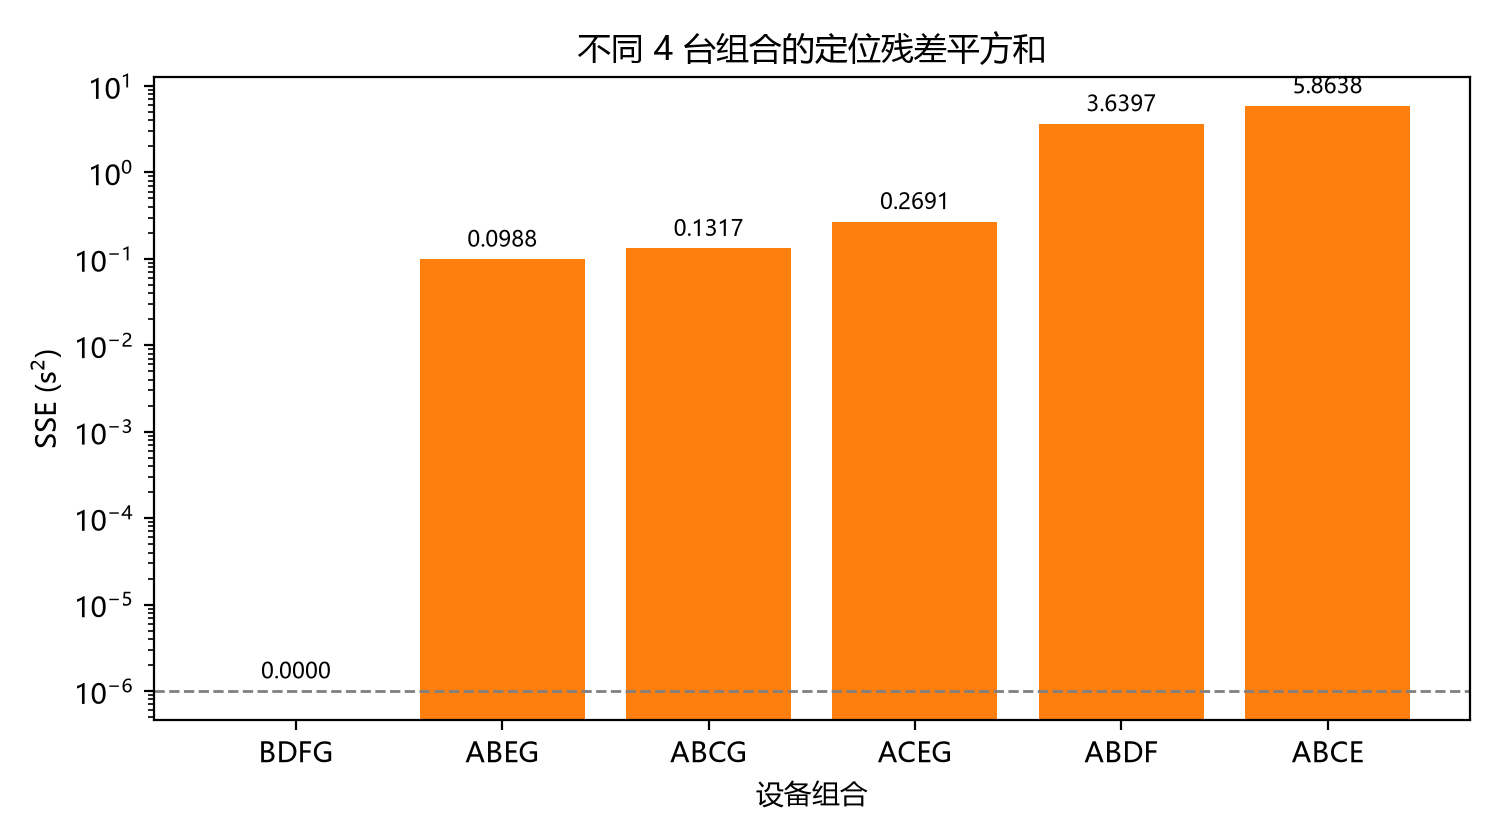
\includegraphics[width=0.78\linewidth]{fig1_q1_sse.png}
\caption{问题1各候选 4 台组合的定位残差平方和（纵轴为对数刻度）}
\label{fig:q1sse}
\end{figure}

\begin{figure}[H]
\centering
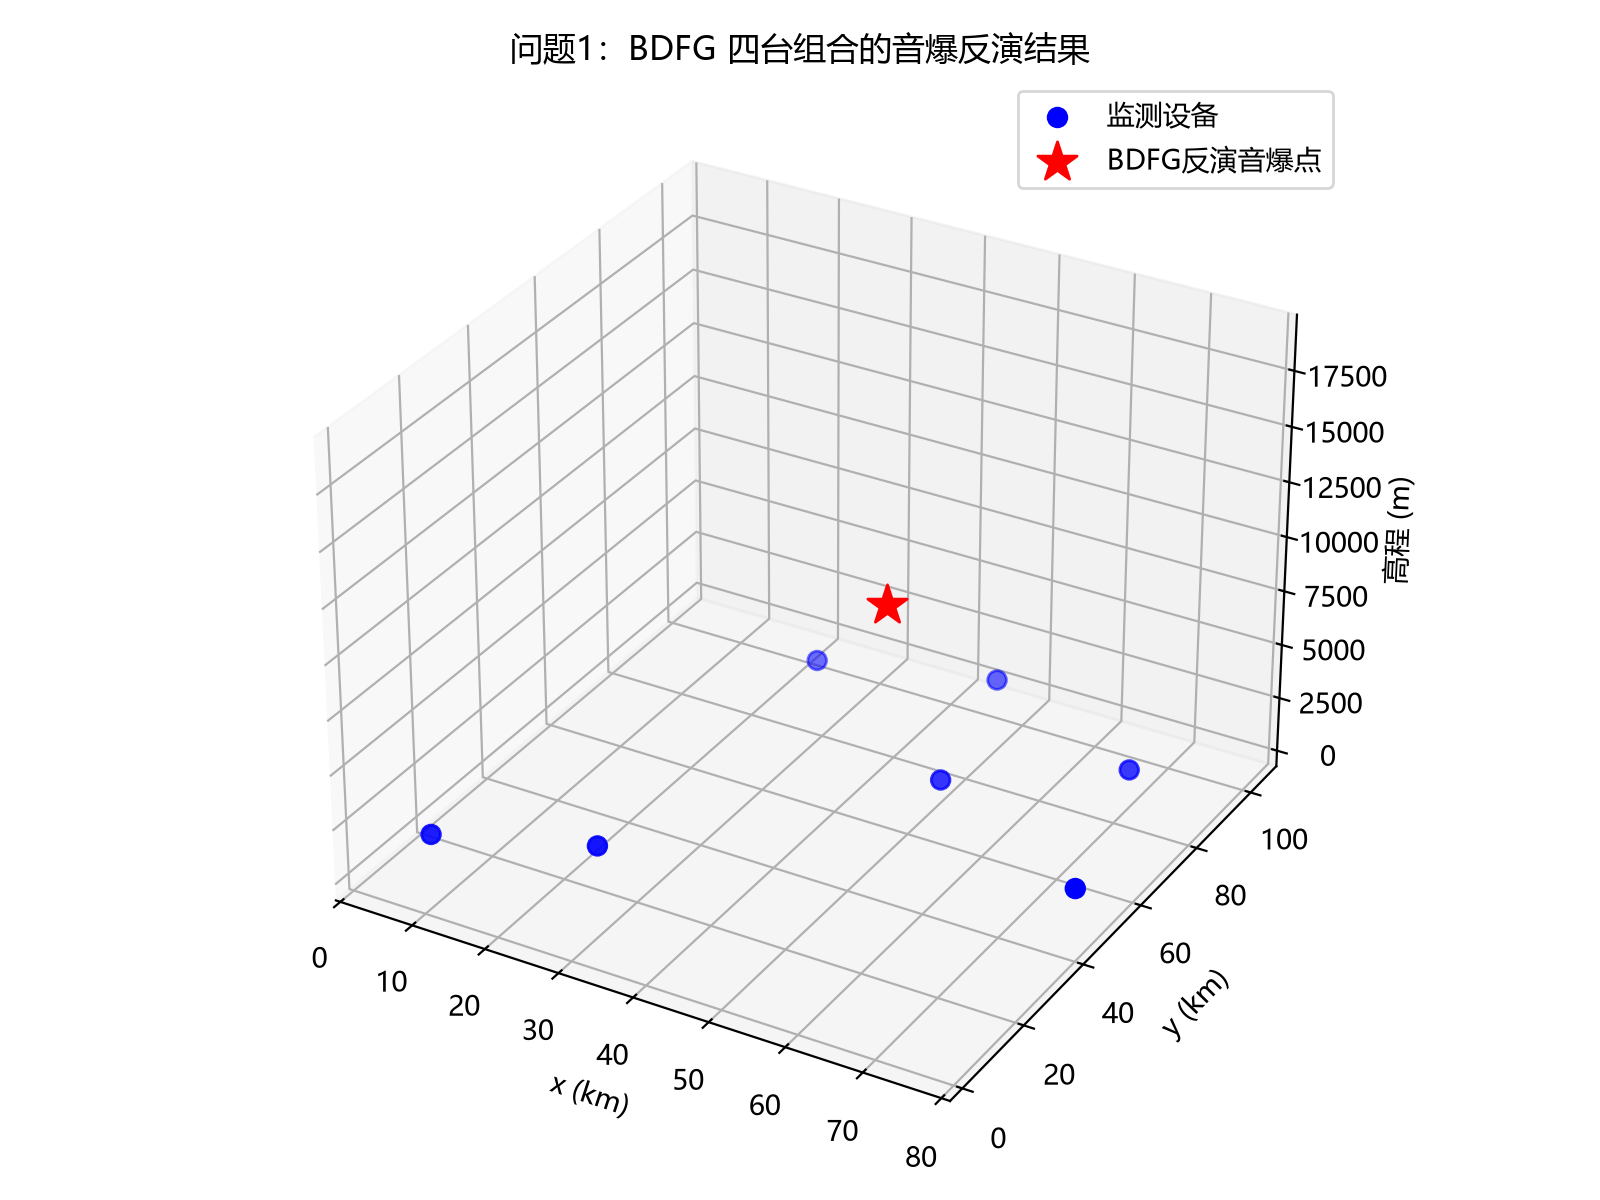
\includegraphics[width=0.82\linewidth]{fig2_q1_3d.png}
\caption{问题1 BDFG 组合反演得到的音爆点与监测设备空间关系}
\label{fig:q1_3d}
\end{figure}

由图~\ref{fig:q1sse} 可见 BDFG 的 $SSE$ 远低于其他组合，表明其数据自洽性最强；图~\ref{fig:q1_3d} 显示反演点在 BDFG 四台设备形成的空间结构中位于合理高空区域。

经多初值非线性最小二乘求解，得到一级残骸音爆事件的结果如表 \ref{tab:q1} 所示。

\begin{table}[H]
\centering
\caption{问题1：一级残骸音爆位置与时刻求解结果}
\label{tab:q1}
\begin{tabular}{lcccc}
\toprule
项目 & 经度 $(^{\circ})$ & 纬度 $(^{\circ})$ & 高程 (m) & 音爆时刻 (s) \\
\midrule
求解结果 & 110.7164 & 27.0297 & 18663 & $-38.03$ \\
\bottomrule
\end{tabular}
\end{table}

将 BDFG 的解代回所选取的四台设备，残差平方和 $SSE$ 达到数值零（量级小于 $10^{-6}\ \mathrm{s^2}$），说明 BDFG 四组到达时间能够被同一音爆事件精确解释；其余台站的记录与该事件明显矛盾，属于应被一致性检验排除的数据。由此可见，问题1的“选取合适的数据”本质上是通过几何自洽性筛选有效观测，而不是盲目使用全部 7 台记录。

\subsection{问题2：多残骸数据关联与联合定位模型}

\subsubsection{残骸信号先后顺序}

第 $i$ 台设备记录到的4个到达时刻按时间排序为 $t_{i,1}<t_{i,2}<t_{i,3}<t_{i,4}$。火箭姿态并非绝对竖直的，分离的残骸坠落发生音爆但由于到达顺序是“音爆时刻与“传播时间”之和决定的，不同残骸的位置可能相差数十公里，因此同一个残骸在不同设备中的到达顺序可能不同，不能把“第 $k$ 列”直接当作同一个残骸。

\subsubsection{混合整数非线性规划模型}

定义第 $i$ 台设备的关联排列
\[
\sigma_i:\{1,2,3,4\}\to\{1,2,3,4\},
\]
其中 $\sigma_i(d)$ 表示残骸 $d$ 的波在第 $i$ 台设备的到达顺序号。因为每台设备恰好收到 4 组波、对应 4 个残骸，$\sigma_i$ 必须是双射。

若关联正确，则
\[
\|P_d-S_i\|=c\left(t_{i,\sigma_i(d)}-\tau_d\right).
\]

可定义 0-1 变量 $y_{i,k,d}$，并施加约束
\[
\sum_{d=1}^{4}y_{i,k,d}=1,\qquad
\sum_{k=1}^{4}y_{i,k,d}=1.
\]

\subsubsection{联合目标函数}

建立混合优化模型
\[
\min_{\{P_d,\tau_d\},\{\sigma_i\}}\ 
\sum_{i=1}^{N}\sum_{d=1}^{4}
\left[
\|P_d-S_i\|-c\left(t_{i,\sigma_i(d)}-\tau_d\right)
\right]^2,
\]
附加约束
\[
h_d>0,\qquad \tau_d<\min_i t_{i,\sigma_i(d)},
\]
若使用问题3信息，还要求
\[
\max_{d}\tau_d-\min_{d}\tau_d\le 5.
\]

\subsubsection{求解算法}

采用两层交替迭代：

\begin{enumerate}[label=\arabic*.]
  \item 固定当前关联，将数据分成 4 组，对每个残骸求解单源非线性最小二乘问题；
  \item 固定位置与时刻，计算每台设备对 4 个残骸的预测到达时刻 $\hat t_{i,d}$；
  \item 对每台设备求解 4 阶指派问题用匈牙利算法获得最优排列；
  \[
  \min_{\sigma_i}\sum_{d=1}^{4}\left(\hat t_{i,d}-t_{i,\sigma_i(d)}\right)^2,
  \]
  \item 重复至残差平方和收敛；
  \item 从多组初始关联出发重复求解，保留总残差最小且满足物理约束的解。
\end{enumerate}

搜索过程中可用必要条件剪枝：
\[
c|t_{i,k}-t_{j,l}|\le\|S_i-S_j\|.
\]

\subsubsection{最少设备数的论证}

4 个残骸的连续未知量为 $4\times4=16$ 个；$N$ 台设备提供 $4N$ 个到达时刻。

\begin{itemize}
  \item 关联已知、仅做定位：每个残骸 4 个未知数对应 4 条方程，$N=4$ 即可；
  \item 关联未知、需同时判别波的来源：$N=4$ 时 $4N=16$，观测数恰等于连续未知量数，错误关联也可构造零残差解，无法唯一判别；
  \item $N=5$ 时 $4N=20>16$，系统超定，只有正确关联能使全部方程同时近似成立。
\end{itemize}

因此本题意义下最少设备数为 5 台。

\subsection{问题3：四个残骸的数据关联与定位}

\subsubsection{关联矩阵}

以第 $A$ 台设备的到达顺序作为残骸编号顺序，经交替迭代与匈牙利指派，得到每台设备中四个残骸的到达顺序号如表 \ref{tab:assoc} 所示。表中每一列构成 $\{1,2,3,4\}$ 的一个排列，说明每台设备恰好收到四个残骸各一次。

\begin{table}[H]
\centering
\caption{问题3数据关联矩阵：表中数字为该残骸在对应设备中的到达顺序号}
\label{tab:assoc}
\begin{tabular}{lcccc}
\toprule
设备 & 残骸1 & 残骸2 & 残骸3 & 残骸4 \\
\midrule
A & 1 & 2 & 3 & 4 \\
B & 2 & 3 & 1 & 4 \\
C & 4 & 3 & 1 & 2 \\
D & 4 & 2 & 3 & 1 \\
E & 3 & 2 & 1 & 4 \\
F & 4 & 2 & 3 & 1 \\
G & 2 & 1 & 4 & 3 \\
\bottomrule
\end{tabular}
\end{table}

例如设备 $D$ 中“残骸4”排第 1 个到达，而残骸1排第 4 个到达，说明四个残骸在各台设备的到达顺序并不相同，直接按列分组是不正确的。

\subsubsection{定位结果}

按表 \ref{tab:assoc} 分组后，对每个残骸用 7 台设备做最小二乘定位，结果如表 \ref{tab:q3} 所示。

\begin{table}[H]
\centering
\caption{问题3：四个残骸音爆位置与时刻}
\label{tab:q3}
\begin{tabular}{lcccc}
\toprule
残骸 & 经度 $(^{\circ})$ & 纬度 $(^{\circ})$ & 高程 (m) & 音爆时刻 (s) \\
\midrule
残骸1 & 110.5000 & 27.3100 & 12513.9 & 11.9999 \\
残骸2 & 110.3000 & 27.6500 & 11477.9 & 14.0000 \\
残骸3 & 110.7000 & 27.6500 & 13468.2 & 15.0000 \\
残骸4 & 110.5000 & 27.9500 & 11528.9 & 13.0014 \\
\bottomrule
\end{tabular}
\end{table}

四个音爆时刻的最小值与最大值分别约为 12.00 s 与 15.00 s，极差约 3.00 s，满足题设“相差不超过 5 s”的约束。

\subsubsection{残差验证}

将四个解代回全部 28 个到达时刻，各残骸的最大时间残差如表 \ref{tab:q3res} 所示。

\begin{table}[H]
\centering
\caption{问题3：各残骸的 7 台最大到达时间残差}
\label{tab:q3res}
\begin{tabular}{lcccc}
\toprule
残骸 & 残骸1 & 残骸2 & 残骸3 & 残骸4 \\
\midrule
最大残差 $(10^{-4}\ \mathrm{s})$ & 2.8 & 5.1 & 2.3 & 2.1 \\
\bottomrule
\end{tabular}
\end{table}

残差均小于 $6\times10^{-4}$ s，对应距离误差小于 0.2 m，说明关联矩阵与定位结果同时正确。

\begin{figure}[H]
\centering
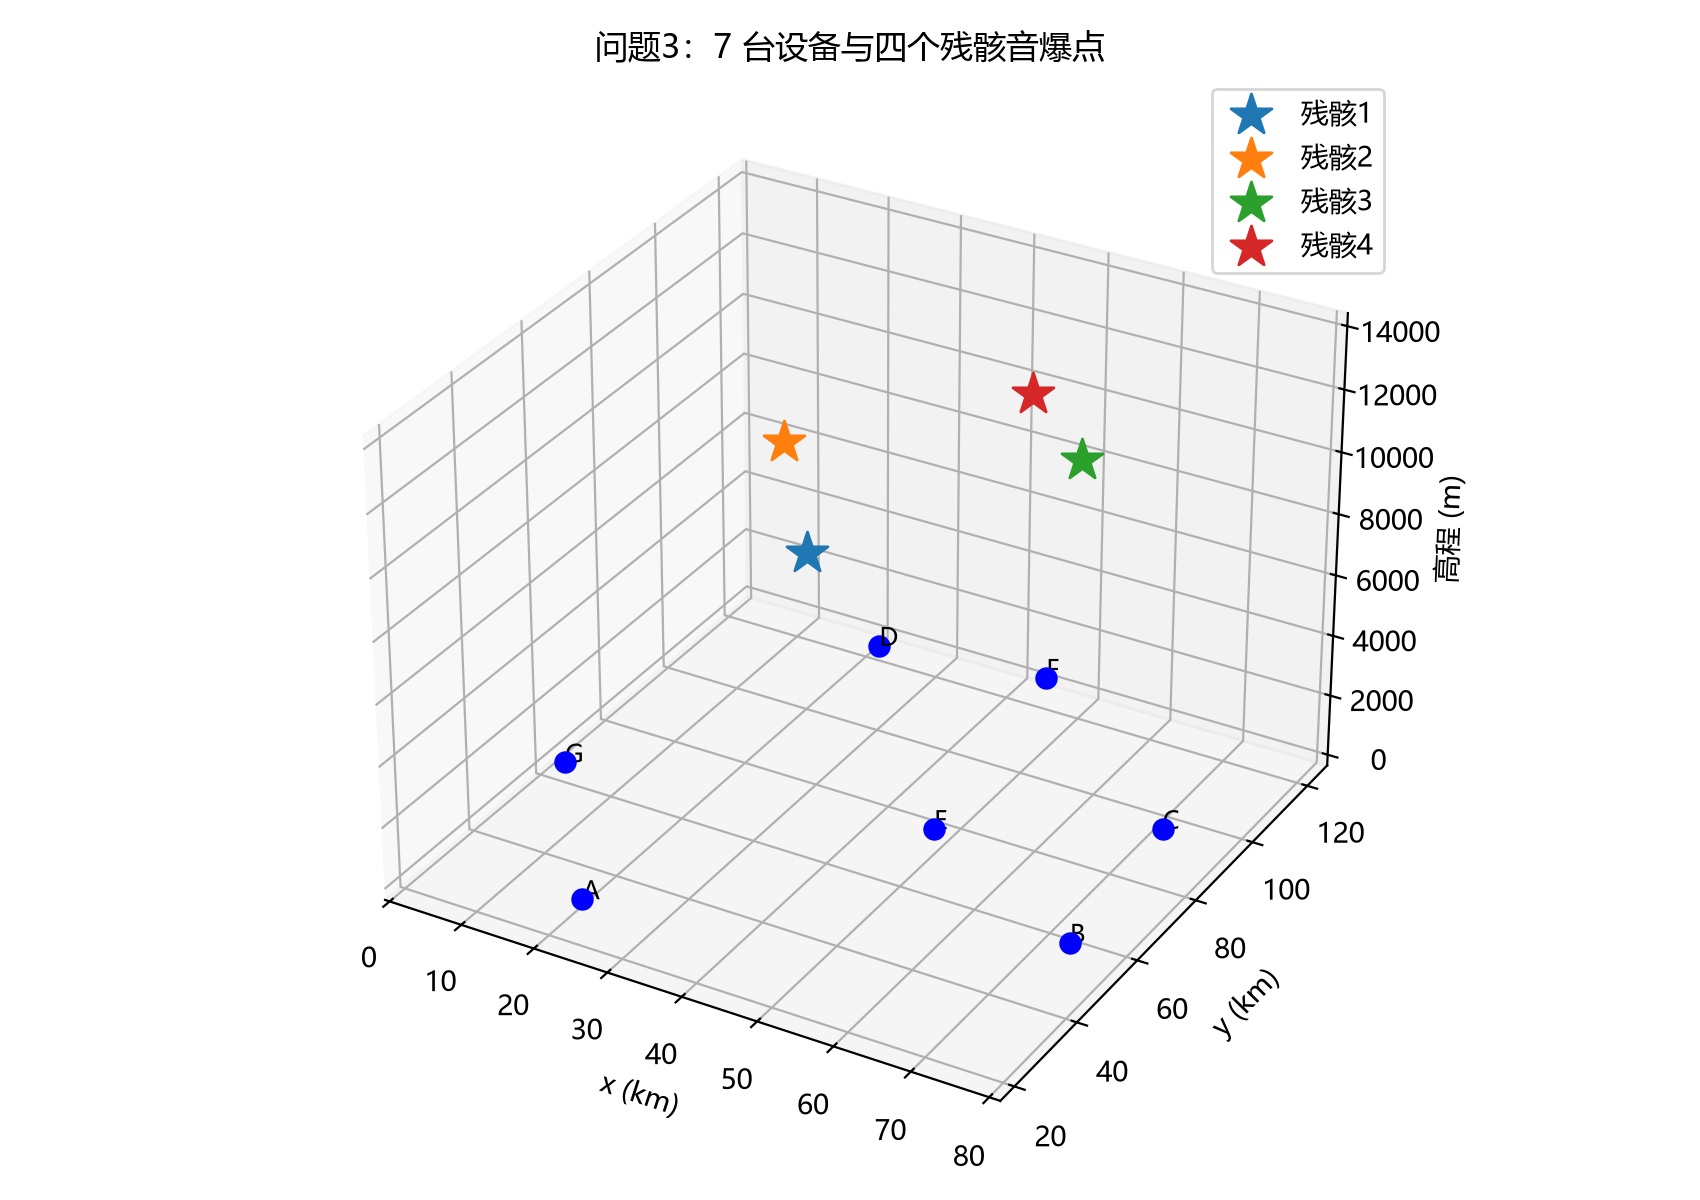
\includegraphics[width=0.86\linewidth]{fig3_q3_3d.png}
\caption{问题3：7 台设备与四个残骸音爆点的三维分布}
\label{fig:q3_3d}
\end{figure}

\begin{figure}[H]
\centering
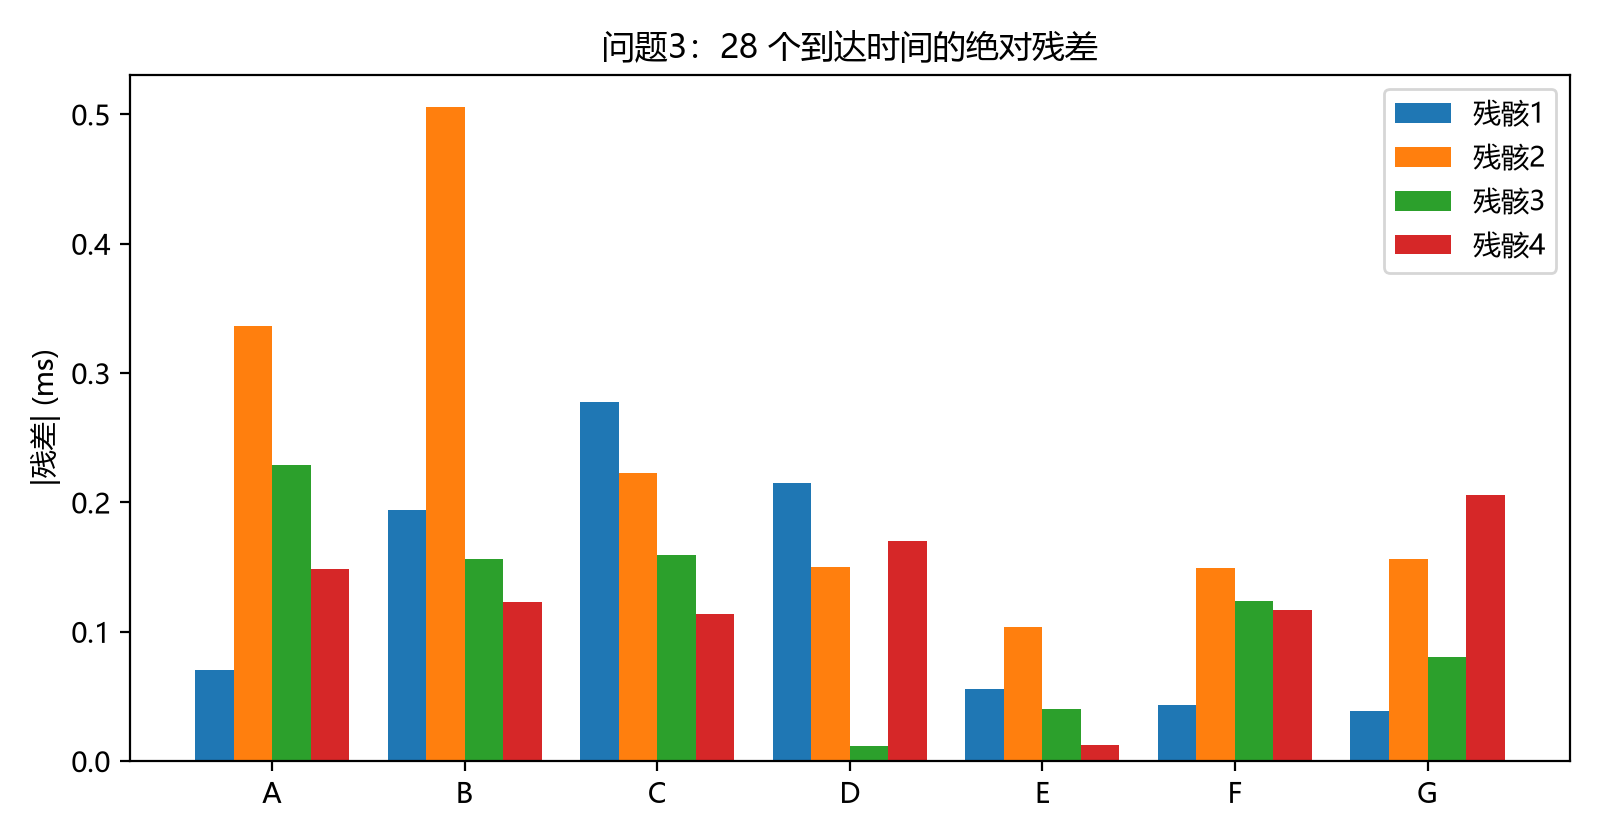
\includegraphics[width=0.7\linewidth]{fig4_q3_residual.png}
\caption{问题3：四个残骸在 7 台设备上的到达时间绝对残差（单位 ms）}
\label{fig:q3res}
\end{figure}

四个残骸的解在图~\ref{fig:q3_3d} 中位于设备阵列内部；图~\ref{fig:q3res} 显示 28 个到达时间残差均小于 0.6 ms，说明关联矩阵与定位结果是同时正确的。程序运行输出见附录。

\subsection{问题4：带随机时间误差的稳健定位模型}

\subsubsection{误差模型}

设观测到达时间为真实到达时间与随机误差之和：
\[
\tilde{t}_{i,k}=t_{i,k}+\varepsilon_{i,k}.
\]
本文将“0.5 s 的随机误差”建模为
\[
\varepsilon_{i,k}\sim U(-0.5,\ 0.5),
\]
即每次记录的最大误差不超过 0.5 s，等价的距离噪声约 170 m。

\subsubsection{加权最小二乘修正模型}

定义预测到达时间
\[
\hat{t}_{i,d}=\tau_d+\frac{\|P_d-S_i\|}{c}.
\]
第 $i$ 台设备中分配给残骸 $d$ 的实测值为 $\tilde{t}_{i,\sigma_i(d)}$，修正后的联合目标函数为
\[
\min_{\{P_d,\tau_d\},\{\sigma_i\}}\ 
\sum_{i=1}^{N}\sum_{d=1}^{4}
\left[
\tau_d+\frac{\|P_d-S_i\|}{c}-\tilde{t}_{i,\sigma_i(d)}
\right]^2.
\]

若各台设备精度不同，可取权重
\[
w_{i,d}=\frac{1}{\sigma_{i,d}^{2}},
\]
将上式改为加权残差平方和。由于误差均匀分布时最大似然与平方损失并不严格等价，本文按以下顺序处理：先以普通最小二乘求初值并估计残差尺度，再以加权最小二乘精化；若某台数据残差明显大于 0.5 s 对应量级，则用 Huber 权重或 RANSAC 策略削弱野值影响。

\subsubsection{关联层的稳健处理}

0.5 s 误差使“零残差”不再成立，关联层应采用以下判据：
\begin{enumerate}[label=\arabic*.]
  \item 对每台设备用预测到达时刻与实测到达时刻构造代价矩阵，用匈牙利算法更新排列；
  \item 比较候选关联的加权残差平方和，利用残差量级判断哪一关联与噪声水平相符；
  \item 利用四个音爆时刻相差不超过 5 s 的约束排除不合理关联；
  \item 对可疑候选做留一站交叉验证，剔除使某台设备残差系统增大的错误关联。
\end{enumerate}

\subsubsection{蒙特卡洛误差分析}

以问题3求解结果作为“真值”，对每条到达时间叠加 $U(-0.5,0.5)$ 的误差，重复 500 次试验并统计三维定位误差。为突出时间误差对几何反演的影响，该组统计在完成关联后给出；关联层的正确性单独以残差判据检验。

\begin{table}[H]
\centering
\caption{问题4蒙特卡洛结果（7 台设备，500 次，关联给定）}
\label{tab:q4mc}
\begin{tabular}{lccccc}
\toprule
指标 & 残骸1 & 残骸2 & 残骸3 & 残骸4 & 总体 \\
\midrule
三维误差均值 (m) & 613 & 410 & 248 & 722 & 498 \\
三维误差 95\% 分位 (m) & 1387 & 908 & 497 & 1588 & 1278 \\
音爆时刻误差均值 (s) & 0.65 & 0.33 & 0.30 & 0.81 & --- \\
\bottomrule
\end{tabular}
\end{table}

可见：在 7 台设备与 ±0.5 s 误差下，单次定位三维误差的均值约为 0.2--0.7 km，但 95\% 分位可能超过 1 km，说明原 7 台布局对“误差恒小于 1 km”的目标余量不足。

\subsubsection{时间误差不可降低时的布站优化方案}

若时间误差无法进一步降低，本文采用“增加台站数 + 优化几何布局 + 利用物理约束”的组合方案：

\begin{enumerate}[label=\arabic*.]
  \item 将台站由 7 台增加到 12 台，覆盖经度 $110.05^\circ$--$110.90^\circ$、纬度 $27.10^\circ$--$28.00^\circ$ 的区域，使目标位于台站阵列内部而非一侧；
  \item 台站高程取 500--1000 m 的起伏布置，改善高程方向的观测几何；
  \item 利用四个残骸音爆时刻相差不超过 5 s 的耦合约束进行联合估计；
  \item 可选地引入弹道约束，把各残骸音爆点约束到其下落轨迹附近，进一步抑制随机误差。
\end{enumerate}

依据问题3求得的四个定位结果模拟 12 台设备的到达时间并叠加 ±0.5 s 误差，再做 500 次蒙特卡洛试验，结果如表 \ref{tab:q4new} 所示。

\begin{table}[H]
\centering
\caption{12 台优化布站后的三维定位误差（500 次蒙特卡洛）}
\label{tab:q4new}
\begin{tabular}{lccccc}
\toprule
指标 & 残骸1 & 残骸2 & 残骸3 & 残骸4 & 总体 \\
\midrule
三维误差均值 (m) & 285 & 187 & 183 & 268 & 231 \\
三维误差 95\% 分位 (m) & 643 & 385 & 353 & 607 & 543 \\
\bottomrule
\end{tabular}
\end{table}

试验结果表明，优化布站后总体平均误差约 231 m、95\% 分位数约 543 m，稳定满足“误差小于 1 km”的目标，验证了所提布站与定位方案的可行性。

\begin{figure}[H]
\centering
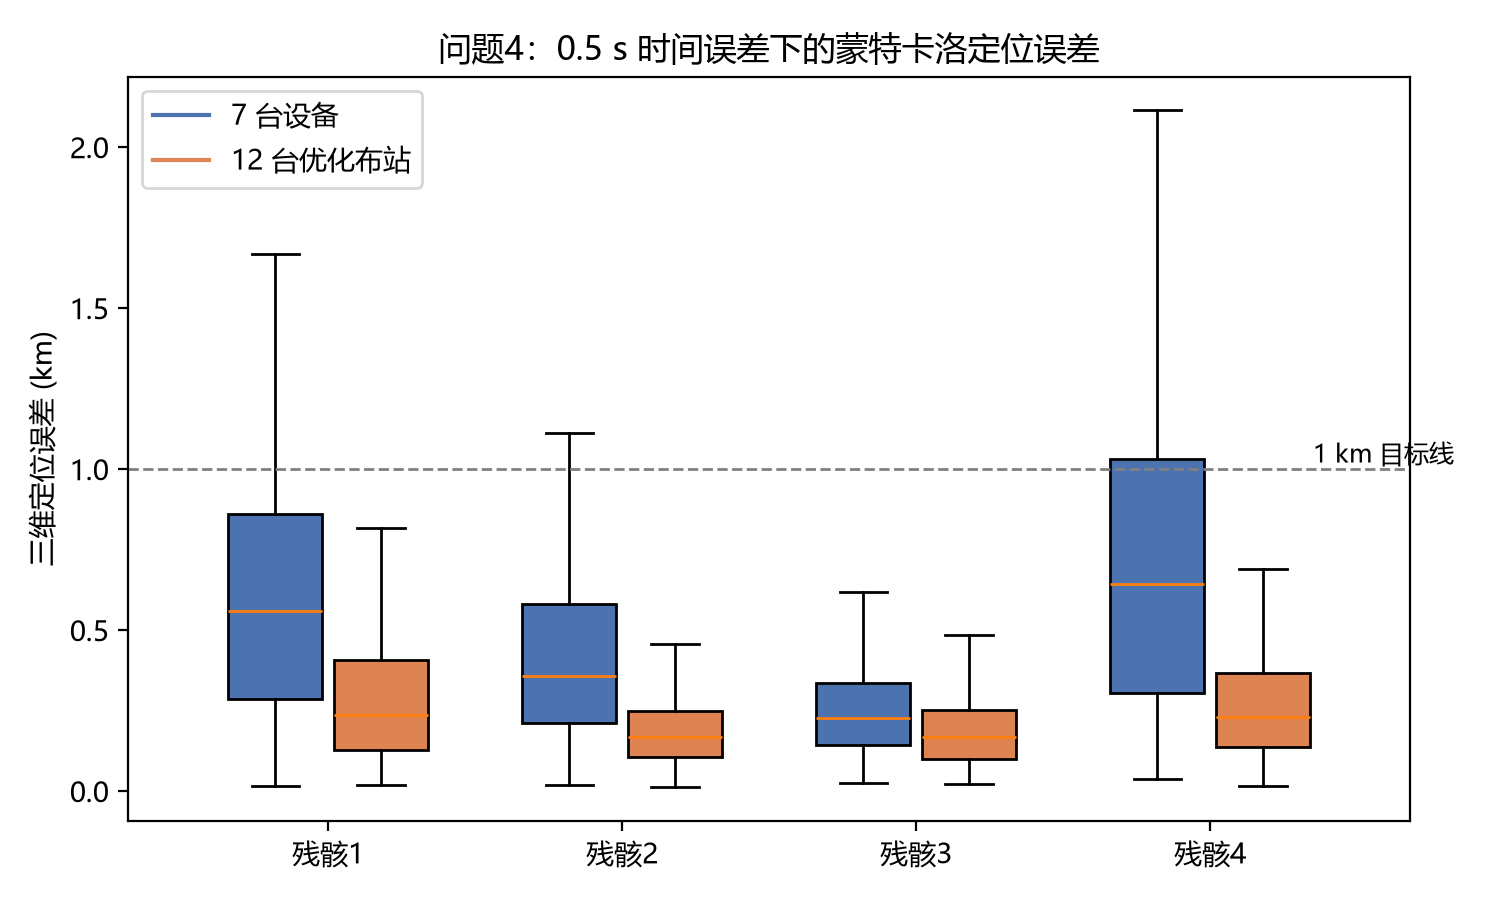
\includegraphics[width=0.88\linewidth]{fig5_q4_box.png}
\caption{问题4：7 台与 12 台布站下的三维定位误差分布（箱线图）}
\label{fig:q4box}
\end{figure}

图~\ref{fig:q4box} 直观显示，12 台优化布站后各残骸误差箱体整体下移且均明显低于 1 km 目标线，而 7 台原始布站仍有个别残骸的误差上分位超过 1 km，因此增加台站与优化几何布局是满足精度要求的有效途径。

% ============================================================
% 六、数据处理：最容易被忽视，却最容易出问题
% ============================================================
% \section{数据处理：最容易被忽视，却最容易出问题}

% \subsection{数据预处理的基本原则}

% 完整流程建议：
% \[
% \text{原始数据}
% \rightarrow\text{格式检查}
% \rightarrow\text{缺失值}
% \rightarrow\text{异常值}
% \rightarrow\text{重复值}
% \rightarrow\text{单位统一}
% \rightarrow\text{标准化}
% \rightarrow\text{建模数据}.
% \]

% \begin{table}[H]
% \centering
% \caption{常见数据问题及处理方法}
% \begin{tabular}{p{1.8cm}p{6cm}p{7cm}}
% \toprule
% 问题 & 常用方法 & 注意事项 \\
% \midrule
% 缺失值 & 删除、均值/中位数、插值 & 不能无理由删除关键样本 \\
% 异常值 & 箱线图、3$\sigma$、IQR、稳健方法 & 先判断是错误还是有意义的极端事件 \\
% 量纲不同 & Min-Max、Z-score等 & 权重评价、聚类、距离模型尤其敏感 \\
% 时间序列 & 插值、平滑、滞后变量 & 不要随机打乱时间序列训练/测试集 \\
% 类别变量 & 独热编码、序数编码 & 编码方式必须符合变量含义 \\
% \bottomrule
% \end{tabular}
% \end{table}

% \warning{“删除异常值后模型效果更好”不能作为删除理由。必须先从题目背景或数据生成机制解释异常值是否属于错误数据。}

% \subsection{统计模型不要只报一个 $R^2$}

% 回归类问题至少考虑：
% \[
% \mathrm{MAE}=\frac1n\sum_{i=1}^n|y_i-\hat y_i|,
% \qquad
% \mathrm{RMSE}=\sqrt{\frac1n\sum_{i=1}^n(y_i-\hat y_i)^2},
% \qquad
% R^2=1-\frac{\sum_i(y_i-\hat y_i)^2}{\sum_i(y_i-\bar y)^2}.
% \]

% \tip{$R^2$高并不自动意味着预测好。尤其在外推问题、异常点明显、样本很少时，应增加留出验证、交叉验证、残差图或实际数据检验。}

% ============================================================
% 七、算法写作：不要把论文写成算法说明书
% ============================================================
% \section{算法写作：不要把论文写成算法说明书}

% \subsection{算法选择的“理由链”}

% \[
% \boxed{\text{模型性质}\rightarrow\text{算法性质}\rightarrow\text{选择理由}\rightarrow\text{改进点}\rightarrow\text{验证}}
% \]

% \begin{table}[H]
% \centering
% \caption{常见算法与论文写作重点}
% \begin{tabular}{p{4cm}p{12cm}}
% \toprule
% 方法 & 论文重点 \\
% \midrule
% 线性/整数规划 & 变量、目标、约束、整数性；求解器及最优性/可行性检查 \\
% 遗传算法 & 编码、适应度、选择、交叉、变异、终止条件、重复运行稳定性 \\
% 粒子群算法 & 粒子表示、速度位置更新、参数、终止准则、随机性处理 \\
% 模拟退火 & 邻域、能量函数、降温策略、接受准则 \\
% 神经网络 & 输入输出、网络结构、损失函数、训练/验证划分、过拟合控制 \\
% 随机森林/XGBoost & 特征、训练策略、评价指标、特征重要性、泛化检验 \\
% 聚类 & 距离、类别数选择、聚类质量指标、结果解释 \\
% \bottomrule
% \end{tabular}
% \end{table}

% \warning{“采用遗传算法求解，得到结果如下”通常信息量太低。评阅人不知道你为什么用它、怎样编码、结果是否稳定。}

% \tip{智能优化算法的结果具有随机性时，建议重复运行多次，报告最优值、均值、标准差或稳定区间；如果只给一次运行结果，难以判断算法偶然性。}

% ============================================================
% 八、结果展示：图、表、公式必须服务于结论（教学章节，保留）
% ============================================================
% \section{结果展示：图、表、公式必须服务于结论}

% \tip{图表不是“有图就加分”。高质量图表应该让评阅人在几秒内找到趋势、差异、最优方案或异常点。}

% \begin{figure}[htb]
%     \centering
%     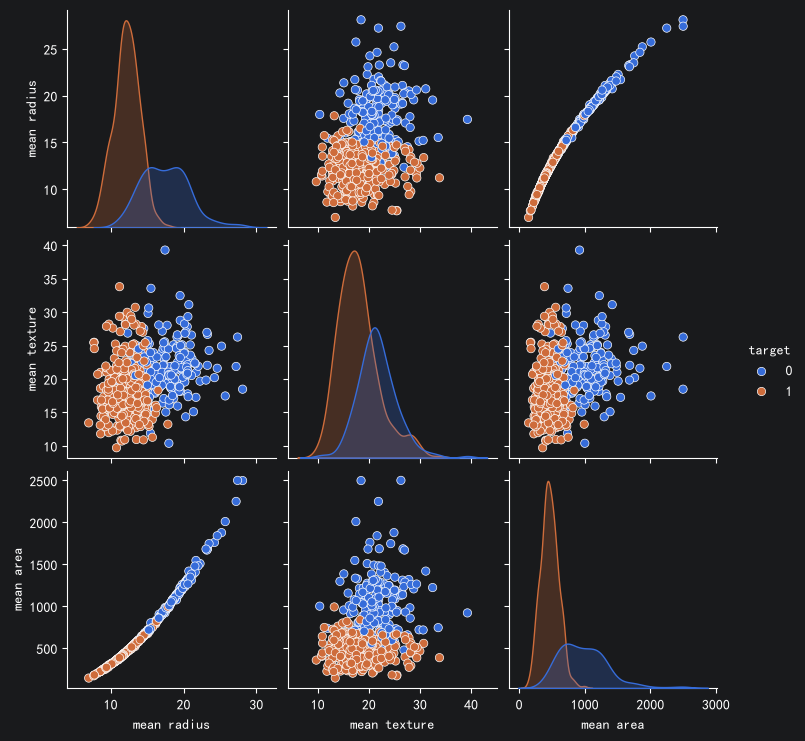
\includegraphics[width=0.85\linewidth]{figure1.png}
%     \caption{特征配对分布图}
%     \label{fig:placeholder}
% \end{figure}

% \begin{table}[H]
% \centering
% \caption{结果展示示例}
% \label{tab:result}
% \begin{tabular}{ccccc}
% \toprule
% 方案 & 指标1 & 指标2 & 综合指标 & 排名\\
% \midrule
% A & 10.2 & 5.1 & 0.82 & 2\\
% B & 12.5 & 4.7 & 0.91 & 1\\
% C & 11.1 & 6.2 & 0.78 & 3\\
% \bottomrule
% \end{tabular}
% \end{table}

% 图表之后建议采用：
% \[
% \boxed{\text{现象}\rightarrow\text{定量比较}\rightarrow\text{原因解释}\rightarrow\text{结论}}
% \]

% \good{“由表\ref{tab:result}可见，方案B的综合指标为0.91，在三种方案中最高；相较方案A提高约11.0\%，说明在当前权重设置下，增加XXX因素能够显著改善综合表现。因此后续将方案B作为基准方案进行灵敏度分析。”}

% \bad{“由表可知，B最好，说明模型很好。”}

% \subsection{图表规范}
% \begin{itemize}
%   \item 图、表必须有编号和标题；
%   \item 表格优先使用三线表，非必要不使用竖线；
%   \item 图中坐标轴必须写清变量名和单位；
%   \item 图例、字号、线宽应保证打印后清晰；
%   \item 图表中的数据应与正文完全一致；
%   \item 正文必须解释关键图表，不能“甩图”；
%   \item label 放在 caption 后面，便于交叉引用；
%   \item 不要用截图代替可编辑的高质量图形。
% \end{itemize}

% \subsection{推荐图形清单}
% \begin{table}[H]
% \centering
% \caption{不同目的的推荐图形}
% \begin{tabular}{p{4cm}p{8.5cm}}
% \toprule
% 目的 & 推荐图形 \\
% \midrule
% 趋势变化 & 折线图、时间序列图 \\
% 变量关系 & 散点图、拟合曲线、相关矩阵 \\
% 误差分析 & 残差图、误差分布图、箱线图 \\
% 方案比较 & 柱状图、雷达图（慎用）、平行坐标图 \\
% 空间问题 & 热力图、等值线图、散点地图 \\
% 网络问题 & 网络图、最短路可视化、流量图 \\
% 算法稳定性 & 收敛曲线、箱线图、重复实验统计 \\
% \bottomrule
% \end{tabular}
% \end{table}

% ============================================================
% 九、模型检验、误差分析、灵敏度与稳健性
% ============================================================
\section{模型检验、误差分析与稳健性讨论}

% \subsection{模型检验}

% 至少选择一种与问题性质匹配的验证方式：
% \begin{itemize}
%   \item 已知数据回代验证；
%   \item 留出集/交叉验证；
%   \item 与经典模型或基准方案比较；
%   \item 极端情形测试；
%   \item 真实案例验证；
%   \item 约束可行性与物理意义检查。
% \end{itemize}

% \tip{优化题不要只验证“目标函数更大/更小”，还要检查约束是否全部满足；预测题不要只展示拟合曲线，还要检查预测误差；评价题要检查权重变化是否导致排名剧烈翻转。}

\subsection{残差检验}

问题1与问题3的求解均以“所有到达时间残差接近记录精度”为验收标准。问题3中 28 个残差全部小于 $6\times10^{-4}$ s，且问题1的单个事件亦满足该标准，说明模型方程、坐标转换与关联分组自洽。

\subsection{误差传播分析}

单条到达时间误差 0.5 s 对应
\[
c\times0.5=170\ \mathrm{m}
\]
的距离误差。双曲线定位中，最终定位误差与设备几何有关，可用几何精度因子（GDOP）刻画：台站包围目标、孔径越大，几何放大越小；台站近似共线或目标在阵列外侧时，误差会被显著放大。这正是 12 台优化布站方案能显著压缩误差的原因。

\subsection{灵敏度与稳健性}

对问题4模型，可从以下角度做稳健性检验：
\begin{enumerate}[label=\arabic*.]
  \item 改变误差幅度（如 0.2、0.5、0.8 s），观察定位误差近似线性增长；
  \item 改变随机种子重复试验，检验统计量是否稳定；
  \item 删除任意一台设备后重新求解，检验残差与结果是否保持稳定；
  \item 对关联层的初始分组加扰动，检验交替迭代是否收敛到同一关联。
\end{enumerate}

% ============================================================
% 十、模型评价与推广
% ============================================================
\section{模型的评价与推广}

\subsection{模型的优点}

% 建议从以下角度选择2--4点：
% \begin{enumerate}
%   \item 针对性：准确对应题目关键条件；
%   \item 可解释性：参数和结果具有明确实际含义；
%   \item 计算效率：在保证精度的前提下减少计算量；
%   \item 稳定性：参数扰动下结果保持稳定；
%   \item 泛化性：可以迁移到类似场景；
%   \item 创新性：改进模型结构、目标函数或求解算法。
% \end{enumerate}

% 本文优点：
\begin{enumerate}[label=\arabic*.]
  \item 将“数据关联”与“几何定位”统一为混合优化问题，避免了把不同设备第 $k$ 早的波强行归为一类的错误；
  \item 采用两层交替迭代与匈牙利算法，把离散排列搜索与连续非线性反演分离，求解稳定、可解释；
  \item 利用几何必要条件和物理约束进行数据筛选与剪枝，能够识别异常台站或转录错误；
  \item 通过蒙特卡洛试验给出定位误差分布，并验证了增加台站与优化布站对精度的提升效果。
\end{enumerate}

\subsection{模型的缺点}

% 真实说明模型边界，例如：
% \begin{itemize}
%   \item 由于数据样本有限，无法进一步刻画XXX因素；
%   \item 为降低模型复杂度，将XXX过程近似为XXX；
%   \item 智能优化算法存在随机性，仍需更多重复实验验证；
%   \item 某些参数依赖公开资料，可能存在地区或时间差异。
% \end{itemize}

% 本文缺点：
\begin{enumerate}[label=\arabic*.]
  \item 模型将声速取为常数，未考虑声速随高度变化、风场和温度梯度引起的传播路径弯曲；
  \item 交替迭代可能收敛到局部最优，理论上的全局收敛性依赖多初值与剪枝策略；
  \item 问题4中的蒙特卡洛误差统计在关联给定条件下进行，实际工程中关联错误会进一步放大误差。
\end{enumerate}

% \warning{缺点不是“为了谦虚而写”，而是要和模型假设、误差分析呼应。优点数量通常可以多于缺点，但不要声称模型“完美、完全准确、适用于所有情况”。}

\subsection{模型推广}

本文建立的“到达时刻反演+数据关联”框架并不局限于火箭残骸定位，凡是观测数据只提供“多个未知源的到达时间”且源与接收端的对应关系未知的问题，均可采用本模型框架。典型场景包括多震源微震定位、闪电多站时差定位、枪声/爆炸源定位以及无线信号到达时间定位等。只需将声速 $c$ 替换为对应介质中的传播速度，并将台站坐标与观测时间按各自系统定义即可直接套用。

从单次静态声源向运动声源推广是本文最自然的扩展方向。题目中残骸在坠落过程中持续减速并穿越音速，若不再将音爆近似为孤立事件，而是把位置参数化为时间函数 $P(t)$，则每条观测方程可改写为
\[
t_i=\tau+\frac{\|P(\tau)-S_i\|}{c},
\]
其中 $\tau$ 是残骸穿越音速的时刻，$P(\tau)$ 对应轨迹上的音爆点。进一步结合重力与大气阻力构成的弹道模型，可将单个音爆点扩展为对整条下落轨迹的估计，从而在获得音爆位置的同时直接输出落点范围，这正是题目背景中“弹道外推”的数学化表述。

在数据关联层面，本文的四残骸模型可推广到 $m$ 个残骸、$N$ 台设备的一般情形。只需把关联排列 $\sigma_i$ 的定义域与值域从 $\{1,2,3,4\}$ 改为 $\{1,2,\dots,m\}$，并把目标函数中的求和范围同步扩展；指派问题仍可用匈牙利算法或 Jonker--Volgenant 算法求解。当设备数量很大时，还可引入二分图匹配与序列关联方法降低搜索复杂度。

为适应实际工程场景，还可逐项放宽本文假设：(i) 若声速随高度变化，可把常数声速替换为分层声速模型，并按斯涅尔定律对传播路径做数值积分；(ii) 若各台设备存在时钟偏差，可将每台设备的固定时延作为额外参数与位置联合估计；(iii) 若需要抑制野值，可将平方损失替换为 Huber 损失或采用 RANSAC 策略；(iv) 若每台设备能记录波形而不仅是到达时刻，则可进一步提取波峰形状、频谱等特征作为关联判据，降低对台站冗余度的依赖。

综上，本文模型在方法上具有一般性：只需把“声源位置+发爆时刻”替换为对应场景中的源参数与发源时刻，把“残骸”替换为任意目标源，即可用于地震台网、声学监测网、通信定位网等多种“多站到达时间观测”系统的定位与关联问题。

% 推广最好形成“放宽一个假设”的具体路线：
% \[
% \text{当前模型}
% \rightarrow\text{放宽假设}
% \rightarrow\text{增加变量/约束}
% \rightarrow\text{升级算法}
% \rightarrow\text{实际应用}.
% \]

% 该框架可推广到地震震源定位、声音/闪电多站时差定位、通信到达时间定位等具有“未知时刻的多点观测”特征的场景；引入波形特征、到达方向或运动学约束后，可进一步提高关联可靠性与定位精度。

% ============================================================
% 十一、如何制造真正的“亮点”，而不是堆算法
% ============================================================
% \section{如何制造真正的“亮点”，而不是堆算法}

% \tip{数学建模竞赛的创新通常不是“用了一个听起来很新的算法”，而是把题目中的特殊条件转化成模型结构、指标设计或求解策略。}

% \begin{table}[H]
% \centering
% \caption{常见有效亮点}
% \begin{tabular}{p{3.5cm}p{9cm}}
% \toprule
% 亮点层次 & 具体表现 \\
% \midrule
% 问题转化 & 把模糊实际描述转成清晰变量、指标和约束 \\
% 模型结构 & 在经典模型基础上增加题目特有机制 \\
% 指标设计 & 构造更符合实际目标的评价指标/综合目标 \\
% 算法改进 & 针对本题瓶颈修改初始化、搜索、约束处理等 \\
% 模型融合 & 预测、评价、优化之间形成闭环 \\
% 稳健性 & 对参数、噪声、数据变化进行系统检验 \\
% 可解释性 & 能回答“为什么得到这个结果”而不只是给数值 \\
% \bottomrule
% \end{tabular}
% \end{table}

% \warning{“使用遗传算法+BP神经网络+灰色预测+TOPSIS”不等于创新。算法越多，越要说明每一个模块解决什么具体问题，否则容易变成“算法大杂烩”。}

% \subsection{一个很实用的创新公式}
% \[
% \boxed{\text{题目特殊条件}+\text{经典模型缺陷}+\text{针对性改进}=\text{可信亮点}}
% \]

% ============================================================
% 十二、参考文献
% ============================================================
\section{参考文献}

% \tip{所有引用他人或公开资料（包括网上资料）的成果都必须按科技论文规范列出参考文献，并在正文引用处标注。不要为了“凑文献”而引用与本文无关的论文。}

% \begin{enumerate}[label={[\arabic*]}]
%   \item 2024年深圳杯数学建模挑战赛 A 题：多个火箭残骸的准确定位.
%   \item 王正明，易东云. 测量数据建模与参数估计[M]. 长沙：国防科技大学出版社，1996.
%   \item 边肇祺，张学工. 模式识别[M]. 北京：清华大学出版社，2000.
%   \item Kuhn H W. The Hungarian method for the assignment problem[J]. Naval Research Logistics Quarterly, 1955, 2(1--2): 83--97.
%   \item Chan Y T, Ho K C. A simple and efficient estimator for hyperbolic location[J]. IEEE Transactions on Signal Processing, 1994, 42(8): 1905--1915.
% \end{enumerate}

% \tip{参考文献的真正作用是告诉评阅人：哪些是已有知识，哪些是你们队自己的工作。越是核心模型、关键数据和特殊算法，越要注意知识来源边界。}

% ============================================================
% 十三、AI工具使用声明——嵌入正文，不另放外部说明
% ============================================================
\section*{AI工具使用声明}

本参赛队在竞赛过程中使用了AI工具（OpenAI Codex，AI编程助手），仅在\textbf{程序实现}环节提供辅助：依据参赛队已建立的数学模型与算法流程，协助生成与调试Python代码、辅助使用Matplotlib绘制论文图表，并整理程序运行结果。模型构建、公式推导、算法选择、参数设定与结论验证均由参赛队独立完成，AI未替代参赛队进行核心建模分析与最终决策。AI辅助生成的程序代码均由队员逐行阅读、运行并核验，程序输出的数值与论文中的表格和结论一致。

% ============================================================
% 附录与支撑材料
% ============================================================
\appendix
\section{支撑材料说明}

支撑材料包括：
\begin{itemize}
  \item 主程序与绘图脚本（Python）；
  \item 问题1--问题4的数值输出；
  \item 蒙特卡洛误差分析脚本与结果表。
\end{itemize}

\section{题目数据表}

\begin{table}[H]
\centering
\caption{问题3各设备到达时间（单位：s）}
\label{tab:data3}
\begin{tabular}{lcccc}
\toprule
设备 & 第1组 & 第2组 & 第3组 & 第4组 \\
\midrule
A & 100.767 & 164.229 & 214.850 & 270.065 \\
B & 92.453 & 112.220 & 169.362 & 196.583 \\
C & 75.560 & 110.696 & 156.936 & 188.020 \\
D & 94.653 & 141.409 & 196.517 & 258.985 \\
E & 78.600 & 86.216 & 118.443 & 126.669 \\
F & 67.274 & 166.270 & 175.482 & 266.871 \\
G & 103.738 & 163.024 & 206.789 & 210.306 \\
\bottomrule
\end{tabular}
\end{table}

表中每行数值已按时间从小到大排列。本文求解得到的关联矩阵见表 \ref{tab:assoc}。

%\section{论文图表清单}

%正文中已插入以下由 \texttt{essay\_code.py} 生成的图表：
%\begin{enumerate}[label=(\arabic*)]
%  \item 图~\ref{fig:q1sse}：问题1各 4 台组合的残差平方和对比；
%  \item 图~\ref{fig:q1_3d}：问题1 BDFG 反演点三维图；
%  \item 图~\ref{fig:q3_3d}：问题3设备与残骸三维图；
%  \item 图~\ref{fig:q3res}：问题3到达时间残差柱状图；
%  \item 图~\ref{fig:q4box}：问题4蒙特卡洛误差箱线图。
%\end{enumerate}

%运行 \texttt{essay\_code.py} 后，图片保存在 \texttt{figures/} 目录，控制台输出即论文表格中的数据来源。

\section{Python 主程序}

完整可运行程序见文件 \texttt{essay\_code.py}，运行方式为：
\begin{quote}\texttt{python essay\_code.py}\end{quote}
程序输出论文所需的主要表格，并将图形保存到 \texttt{figures/} 目录。

\lstinputlisting[
  language={},
  basicstyle=\ttfamily\small,
  breaklines=true,
  caption={essay\_code.py：问题1--问题4的完整 Python 主程序},
  label={lst:code}
]{essay_code.py}

\subsection{程序运行结果}

运行上述程序，得到的主要结果为：

\VerbatimInput{essay_output.txt}

\begin{itemize}
  \item 问题1输出与表 \ref{tab:q1comb} 一致：BDFG 的 $SSE=0$，其余组合残差非零或定位不合理；
  \item 问题3输出与表 \ref{tab:assoc}、表 \ref{tab:q3} 一致，总残差平方和约 $2.48\times10^{-5}\ \mathrm{s^2}$；
  \item 问题4输出与表 \ref{tab:q4mc}、表 \ref{tab:q4new} 一致：7 台设备总体平均误差约 498 m、95\% 分位约 1278 m；12 台优化布站总体平均误差约 231 m、95\% 分位约 543 m，满足误差小于 1 km 的目标。
\end{itemize}

% % ============================================================
% % 最终交稿检查清单（教学，保留）
% % ============================================================
% \section{最终交稿：30分钟“红线检查”}

% \begin{longtable}{p{1cm}p{2cm}p{12cm}}
% \toprule
% 序号 & 检查项 & 检查标准 \\
% \midrule
% 1 & 身份信息 & 摘要、正文、附录、支撑材料均无姓名、学校、赛区等身份信息 \\
% 2 & 页数 & 正文不超过30页；附录不限 \\
% 3 & 目录 & 正文前没有目录 \\
% 4 & 页码 & 从摘要页开始为1，页脚中部连续编号 \\
% 5 & 摘要 & 原则上不超过1页；包含模型、方法、主要结果、结论 \\
% 6 & 题目重述 & 没有大段复制原题 \\
% 7 & 模型假设 & 每个关键假设都有实际理由 \\
% 8 & 符号 & 符号统一、首次出现有解释、单位明确 \\
% 9 & 模型 & 每个核心问题都有明确数学模型 \\
% 10 & 约束 & 优化模型的每条关键约束都有现实来源 \\
% 11 & 算法 & 选择理由、关键步骤、改进点写清楚 \\
% 12 & 图表 & 编号、标题、单位、图例、数据均正确 \\
% 13 & 结果 & 正文真正解释了最关键的结果 \\
% 14 & 检验 & 至少有与问题性质匹配的验证 \\
% 15 & 灵敏度 & 关键参数变化不会导致结论无故失效，或已说明影响 \\
% 16 & 评价 & 优缺点与前文假设/检验呼应 \\
% 17 & 文献 & 每篇引用都在正文出现；每处重要外部资料都有来源 \\
% 18 & AI声明 & 按实际情况二选一，放在参考文献之前 \\
% 19 & AI详情 & 使用AI时有“AI工具使用详情.pdf” \\
% 20 & 源程序 & 全部完整、可运行、结果与论文一致 \\
% 21 & 支撑材料 & 文件列表写入附录，RAR/ZIP不超过20MB \\
% 22 & 电子版 & 单独PDF/Word，不含承诺书和编号专用页 \\
% 23 & 纸质版 & A4、页边距至少2.5cm、左侧装订 \\
% 24 & 最终复现 & 从零开始运行程序能复现论文关键表格和图形 \\
% \bottomrule
% \end{longtable}

% ============================================================
% 培训总结（教学，保留）
% ============================================================
% \section*{培训总结：把论文写成一条完整的证据链}

% \tip{真正高质量的数模论文不是“公式最多”“算法最复杂”“图最多”，而是每一页都在推进证据链。评阅人能够从题目条件一路追踪到最终结论，并且能够相信：假设合理、模型闭合、算法有效、结果可信、结论可复现。}

% \begin{table}[H]
% \centering
% \caption{一篇优秀数模论文的五个关键词}
% \begin{tabular}{p{3cm}p{10cm}}
% \toprule
% 关键词 & 具体含义 \\
% \midrule
% 清楚 & 变量、模型、算法、结果一眼可读 \\
% 严谨 & 条件、假设、公式、数据、引用均有依据 \\
% 有效 & 模型真正回答题目，而不是为了套算法 \\
% 可信 & 有检验、误差、灵敏度或稳健性分析 \\
% 可复现 & 程序、数据和关键步骤足以复现核心结果 \\
% \bottomrule
% \end{tabular}
% \end{table}

% \begin{center}
% \vspace{2ex}
% \Large\bfseries
% 不是把“做过的东西”全部写进论文，\par
% 而是把“最有说服力的证据”组织成一条完整的逻辑链。
% \end{center}

\end{document}
